\documentclass[aspectratio=169]{beamer}

\usepackage[utf8]{inputenc}

\usepackage{amsfonts}
\usepackage{amsmath}
\usepackage{color}
\usepackage{listings}
\usepackage{tikz}
\usepackage{hyperref}

\newif\ifnotes
  \notestrue
%  \notesfalse

\newif\iftransitions
 \transitionstrue
% \transitionsfalse

\newif\iffast
% \fasttrue
  \fastfalse

\ifnotes
\usepackage{pgfpages}
\setbeameroption{show notes}
\setbeameroption{show notes on second screen=right}
\fi

\usetheme{Rochester}
\usecolortheme{beaver}

\addtobeamertemplate{navigation symbols}{}{%
    \usebeamerfont{footline}%
    \usebeamercolor[fg]{footline}%
    \hspace{1em}%
    \insertframenumber/\inserttotalframenumber
}

\lstloadlanguages{C++}
    \lstset{%
        language={C++},
        basicstyle=\ttfamily,
        keywordstyle=\color{blue},
        showstringspaces=false,
        escapechar={§},
        escapeinside={(*@}{@*)}
    }

\lstdefinestyle{cpp20}{language={C++},
  morekeywords={noexcept,co_await,co_return,co_yield,requires,consteval,constinit,concept,module,export,import}
}

\lstdefinestyle{cmake}{
  morekeywords={add_executable,add_library,cmake_minimum_required,project,target_include_directories,target_link_libraries,target_sources}
}

\tikzstyle{every picture}+=[remember picture]

\newcommand{\cpause}{\iftransitions \pause \fi}

\newcommand{\cuncover}[2]{\iftransitions \uncover<#1>{#2} \else #2 \fi}

\newcommand{\tmrk}[2]{\tikz[baseline,inner sep=0]\node[anchor=base](#1){#2};}

\title{C++ Modules - Getting Started Today}
\author{Andreas Weis}
\institute{Woven by Toyota}

\date{MUC++ September 2023}
\titlegraphic{
\includegraphics[height=.15\textheight]{resources/mucpp-logo-128x128.png}}

\iffalse
Modules have been one of the most highly anticipated features of C++20. Unfortunately, it was also the language feature that took the longest to become widely available for developers to use. This year for the first time we see broad support for the feature in all major compilers and mainstream build system support through CMake. The goal of this talk is to provide you with all the basic knowledge to allow you getting started with C++20 modules today.

We will take a look at how modules change the build process and why it took so long to implement them. We will take a tour of the essentials of the named modules mechanism and explore the new best practices for physical code structure in a modules-based code base, including how to set up a build with CMake. And last but not least, we will discuss different options for interacting with existing header-based code.

The talk will focus above all else on practicality: We will only be covering features that are widely available for use today with the latest compilers and build tools. We will give special attention to the areas where the design practices for modules differ from the familiar header-based approach and address common misconceptions and pitfalls that are typical among developers first encountering the feature. No prior knowledge of modules is required.

Outline:
* Modules "Hello World" example
* Differences module interfaces vs header files
* Understanding the build process for modules
* Build system support with CMake and Ninja/MSBuild
* Modules with static and shared libraries
* Best practices for code structure with modules
* Migrating legacy code
* The modularized standard library
* Wrapping third-party code in named modules interfaces

Comments:
This talk aims for breadth not depth. The intention is to give an overview of all the essential topics that are useful when picking up modules for the first time, while not going into as much detail as the more specialized talks we saw at CppCon in the past.
\fi

\begin{document}

\frame{\titlepage}

\iftrue %crop
\fi

\begin{frame}[fragile]
  \frametitle{About me - Andreas Weis (he/him)}

  \begin{itemize}
    \setlength\itemsep{1.5em}

    \item \href{https://stackoverflow.com/users/577603/comicsansms}{
\includegraphics[height=.05\textheight]{resources/so-icon.png}} \href{https://github.com/ComicSansMS}{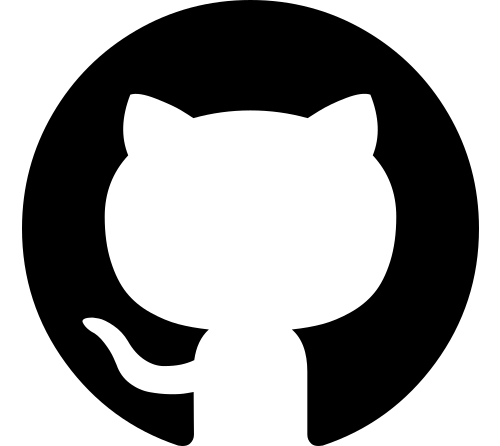
\includegraphics[height=.05\textheight]{resources/github-icon.png}} \includegraphics[height=.05\textheight]{resources/discord-icon.png} ComicSansMS

    %\item \href{https://twitter.com/DerGhulbus/}{
\includegraphics[height=.05\textheight]{resources/twitter-icon.png} @DerGhulbus}

    \item 
\includegraphics[height=.05\textheight]{resources/meetup-icon.png} Co-organizer of the \href{https://www.meetup.com/MUCplusplus/}{Munich C++ User Group}

    \item Currently working as a Vehicle Architect for Woven by Toyota \includegraphics[height=.1\textheight]{resources/woven_toyota_logo.png}

  \end{itemize}
\end{frame}

\iffalse
\begin{frame}
  \frametitle{Overview}
  \begin{itemize}
    \item Categorization of precondition violations
    \item Leveraging the type system to prevent precondition violations
    \item Techniques for restricting access to data
    \item Techniques for restricting control flow
    \end{itemize}
\end{frame}
\fi

\begin{frame}[fragile]
  \frametitle{A familiar example...}
  
  --- \textit{File:} \texttt{my\_function.hpp}
  \begin{lstlisting}[style=cpp20]
char const* my_function();
  \end{lstlisting}

  --- \textit{File:} \texttt{my\_function.cpp}
  \begin{lstlisting}[style=cpp20]
char const* my_function() {
  return "Hello from function!";
}
  \end{lstlisting}

  \cpause
  --- \textit{File:} \texttt{main.cpp}
  \begin{lstlisting}[style=cpp20]
#include <my_function.hpp>
#include <print>

int main() {
  std::println("{}", my_function());
}
  \end{lstlisting}
  
  \note{
  }
\end{frame}

\begin{frame}[fragile]
  \frametitle{\texttt{\#include} can happen anywhere}
  --- \textit{File:} \texttt{a.hpp}
  \begin{lstlisting}[style=cpp20]
inline int my_function
#include <a_impl.hpp>
  \end{lstlisting}

  --- \textit{File:} \texttt{a\_impl.hpp}
  \begin{lstlisting}[style=cpp20]
{
  return 42;
}
  \end{lstlisting}
\end{frame}


\begin{frame}[fragile]
  \frametitle{Including files twice does not work}
  
  --- \textit{File:} \texttt{a.hpp}
  \begin{lstlisting}[style=cpp20]
class A {};
  \end{lstlisting}

  --- \textit{File:} \texttt{main.cpp}
  \begin{lstlisting}[style=cpp20]
#include <a.hpp>
#include <a.hpp>  // redefiniton error!

int main() {
}
  \end{lstlisting}
\end{frame}

\begin{frame}[fragile]
  \frametitle{Included files are not isolated from the surrounding state}
  
  --- \textit{File:} \texttt{a.hpp}
  \begin{lstlisting}[style=cpp20]
class A {
private:
  char const* u_cant_touch_this() {
    return "Preprocessor hits me so hard";
  }
};
  \end{lstlisting}
  \cpause
  --- \textit{File:} \texttt{main.cpp}
  \begin{lstlisting}[style=cpp20]
#define private public
#include <a.hpp>
#undef private
int main() {
  std::println("{}", A{}.u_cant_touch_this());
}
  \end{lstlisting}
\end{frame}

\begin{frame}[fragile]
  \frametitle{Included files do not need to be self-contained}
  
  --- \textit{File:} \texttt{a.hpp}
  \begin{lstlisting}[style=cpp20]
class A {
  std::vector<int> numbers;
};
  \end{lstlisting}

  --- \textit{File:} \texttt{main.cpp}
  \begin{lstlisting}[style=cpp20]
#include <vector>
#include <a.hpp>

int main() {
}
  \end{lstlisting}
\end{frame}

\begin{frame}[fragile]
  \frametitle{Include files are compiled again for each translation unit}
  
    --- \textit{File:} \texttt{a.cpp}
  \begin{lstlisting}[style=cpp20]
#include <massive_header.hpp>
  \end{lstlisting}

  --- \textit{File:} \texttt{b.cpp}
  \begin{lstlisting}[style=cpp20]
#include <massive_header.hpp>
  \end{lstlisting}
\end{frame}

\begin{frame}
  \frametitle{Before we dive into modules...}
  
  \begin{center}
  \huge{Disclaimer}
  \end{center}
\end{frame}


\begin{frame}[fragile]
  \frametitle{Hello Modules!}
  
  --- \textit{File:} \texttt{module.cpp}
  \begin{lstlisting}[style=cpp20]
(*@\tmrk{exp01}{}@*)export module my_module;(*@\tmrk{exp02}{}@*)

export char const* my_function() {
  return "Hello Modules!";
}
  \end{lstlisting}
  
  \cuncover{2-}{\tikz[overlay]\filldraw[blue, opacity=0.3] ([shift={(0,-0.5ex)}]exp01) rectangle ([shift={(0,2ex)}]exp02);}

  \cpause
  \cpause

  --- \textit{File:} \texttt{main.cpp}
  \begin{lstlisting}[style=cpp20]
(*@\tmrk{imp01}{}@*)import my_module;(*@\tmrk{imp02}{}@*)
#include <print>

int main() {
  std::println("{}", my_function());
}
  \end{lstlisting}

  \cuncover{4-}{\tikz[overlay]\filldraw[blue, opacity=0.3] ([shift={(0,-0.5ex)}]imp01) rectangle ([shift={(0,2ex)}]imp02);}

  \note{
    \begin{itemize}
      \item Module name is different from file name!
      \item Module does not introduce a namespace
    \end{itemize}
  }
\end{frame}

\begin{frame}[fragile]
  \frametitle{Exporting things}
  
  \begin{lstlisting}[style=cpp20]
// functions
export int getNumber();
  \end{lstlisting}
  \cpause
  \begin{lstlisting}[style=cpp20]
// types
export class SomeType;
  \end{lstlisting}
  \cpause
  \begin{lstlisting}[style=cpp20]
// templates
export template<typename T>
T combine(T n1, T n2);
export template<typename T>
class MyTemplatedType;
  \end{lstlisting}
  
  \note{
  We are exporting declarations!
  }
\end{frame}

\begin{frame}[fragile]
  \frametitle{Exporting things}

  \begin{lstlisting}[style=cpp20]
export namespace a {
  void is_exported();
}
namespace a {
  void is_not_exported();
}
  \end{lstlisting}
  \cpause
  \begin{lstlisting}[style=cpp20]
namespace a {
  void will_be_exported_in_b();
}
export namespace b {
  export using a::will_be_exported_in_b;
}
  \end{lstlisting}
\end{frame}

\begin{frame}[fragile]
  \frametitle{Exporting things}
  
  --- \textit{File:} \texttt{module1.cpp}
  \begin{lstlisting}[style=cpp20]
export module A;

export int foo() { return 42; }
  \end{lstlisting}
  --- \textit{File:} \texttt{module2.cpp}
  \begin{lstlisting}[style=cpp20]
export module B;

export import A;
  \end{lstlisting}
  \cpause
  --- \textit{File:} \texttt{main.cpp}
  \begin{lstlisting}[style=cpp20]
import B;
int main() {
  return foo();
}
  \end{lstlisting}
\end{frame}

\begin{frame}[fragile]
  \frametitle{Not exported does not mean unreachable}

  --- \textit{File:} \texttt{module.cpp}
  \begin{lstlisting}[style=cpp20]
export module m;
class NotExported { int i = 42; };
export NotExported getNotExported() { return {}; }
  \end{lstlisting}
  \cpause
  --- \textit{File:} \texttt{main.cpp}
  \begin{lstlisting}[style=cpp20]
import m;
int main() {
  int const ii = getNotExported().i;
}
  \end{lstlisting}
  \cpause
  This is not new!
  \begin{lstlisting}[style=cpp20]
auto getS() { struct S { int i = 42; }; return S{}; }
  \end{lstlisting}
\end{frame}

\begin{frame}
  \frametitle{Daniela Engert - The three secret spices of C++ Modules - \\ Visibility, Reachability, Linkage}
  \begin{center}
    \href{https://www.youtube.com/watch?v=l_83lyxWGtE}
    {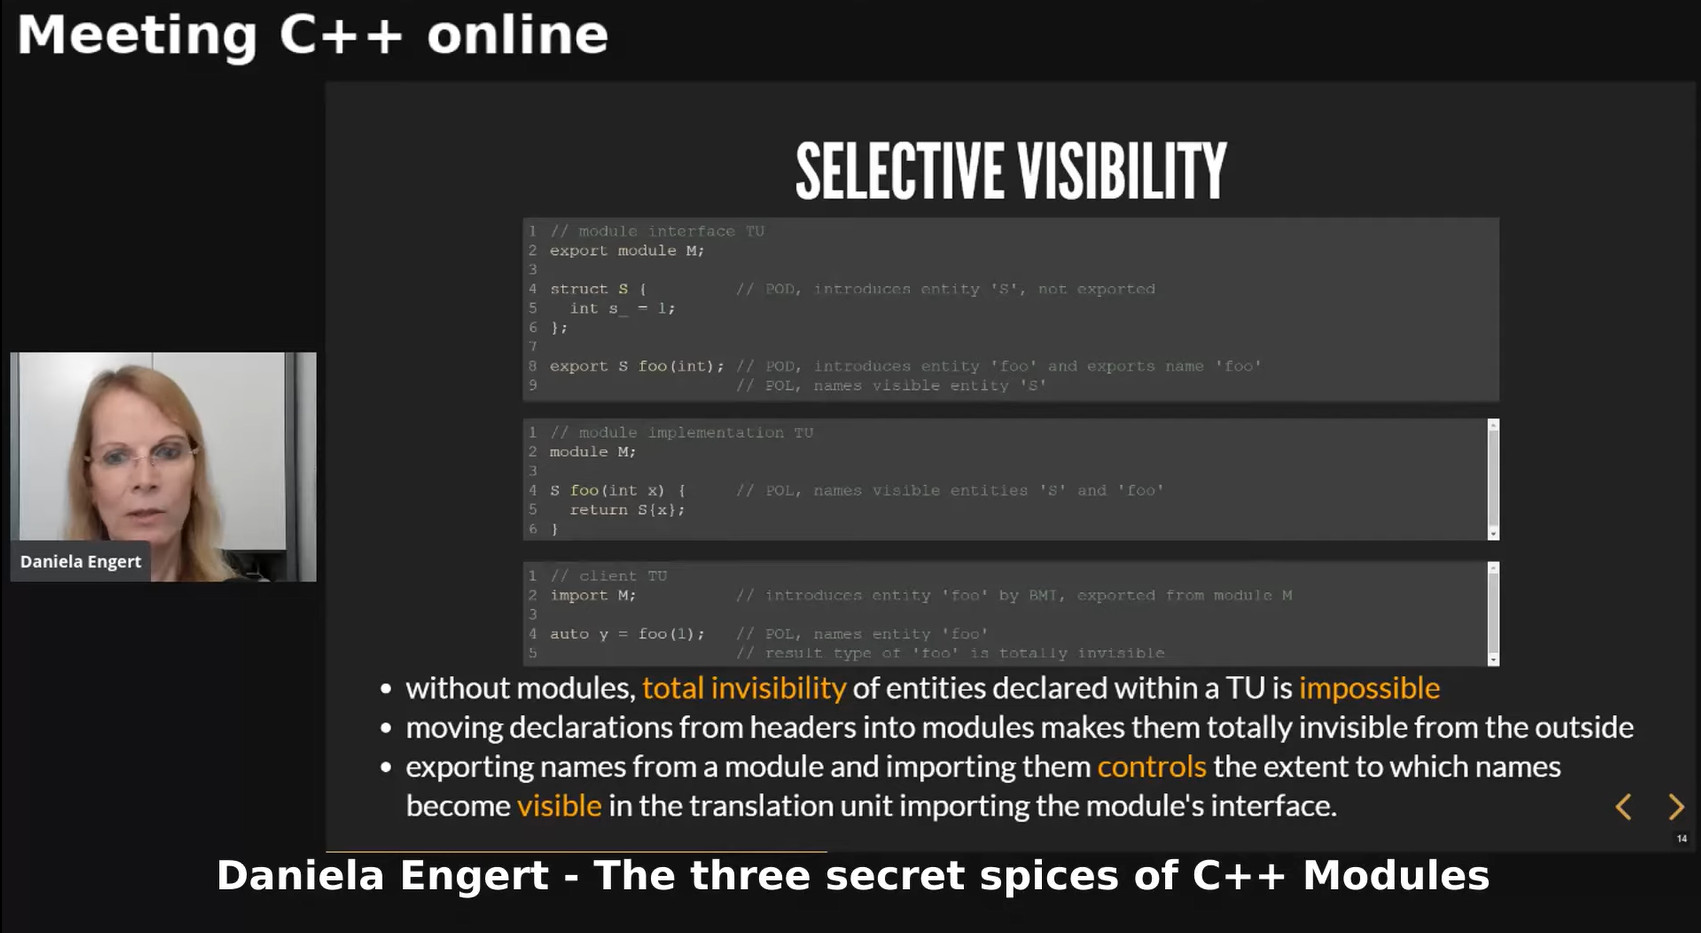
\includegraphics[height=.8\textheight]{modulesgfx/engert_three_spices.jpg}}
  \end{center}
\end{frame}

\begin{frame}[fragile]
  
  \only<1>{\frametitle{Primary Module Interface Unit}}
  \only<2->{\frametitle{Module Implementation Unit}}
  
  --- \textit{File:} \texttt{my\_module.cpp}
  \begin{onlyenv}<1>
  \begin{lstlisting}[style=cpp20]
export module my_module;

export char const* my_function() {
  return "Hello Modules!";
}
  \end{lstlisting}
  \end{onlyenv}
  \begin{uncoverenv}<2->
  \begin{lstlisting}[style=cpp20]
export module my_module;

export char const* my_function();
  \end{lstlisting}
  --- \textit{File:} \texttt{my\_module\_impl.cpp}
\begin{lstlisting}[style=cpp20]
(*@\tmrk{a020}{}@*)module my_module;(*@\tmrk{b020}{}@*)

char const* my_function() {
  return "Hello Modules!";
}
  \end{lstlisting}
  \end{uncoverenv}
  
  \cuncover{3-}{\tikz[overlay]\filldraw[blue, opacity=0.3] ([shift={(0,-0.5ex)}]a020) rectangle ([shift={(0,2ex)}]b020);}
  
  \note{
  \begin{itemize}
  \item Primary, because there can be only one for each module name
  \item By default, put everything in primary module
  \item Export only on declaration in interface, not in implementation; compile error otherwise
  \item Like Headers, as many implementations as we want
  \item Unlike Headers, no need to split
  \item Impl can change without rebuilding clients of interface
  \end{itemize}
  }
\end{frame}

\begin{frame}[fragile]
  \frametitle{Module Interface Partitions}
  
  --- \textit{File:} \texttt{my\_module.cpp}
  \begin{lstlisting}[style=cpp20]
export module m;

(*@\tmrk{a030}{}@*)export import :pinky;(*@\tmrk{b030}{}@*)
(*@\tmrk{a031}{}@*)export import :the_brain;(*@\tmrk{b031}{}@*)
  \end{lstlisting}
  
  --- \textit{File:} \texttt{my\_module\_p1.cpp}
  \begin{lstlisting}[style=cpp20]
export module (*@\tmrk{a032}{}@*)m:pinky(*@\tmrk{b032}{}@*);
export void narf() {}
  \end{lstlisting}
  
  --- \textit{File:} \texttt{my\_module\_p2.cpp}
  \begin{lstlisting}[style=cpp20]
export module (*@\tmrk{a033}{}@*)m:the_brain(*@\tmrk{b033}{}@*);
export void take_over_the_world() {}
(*@\tmrk{a034}{}@*)struct SecretMasterplan {}(*@\tmrk{b034}{}@*);
  \end{lstlisting}
  
  \only<3>{\tikz[overlay]\filldraw[blue, opacity=0.3] ([shift={(0,-0.5ex)}]a030) rectangle ([shift={(0,2ex)}]b030);}
  \only<3>{\tikz[overlay]\filldraw[blue, opacity=0.3] ([shift={(0,-0.5ex)}]a031) rectangle ([shift={(0,2ex)}]b031);}
  \only<2>{\tikz[overlay]\filldraw[blue, opacity=0.3] ([shift={(0,-0.5ex)}]a032) rectangle ([shift={(0,2ex)}]b032);}
  \only<2>{\tikz[overlay]\filldraw[blue, opacity=0.3] ([shift={(0,-0.5ex)}]a033) rectangle ([shift={(0,2ex)}]b033);}
  \only<4>{\tikz[overlay]\filldraw[blue, opacity=0.3] ([shift={(0,-0.5ex)}]a034) rectangle ([shift={(0,2ex)}]b034);}
  
  \note{
  \begin{itemize}
  \item Split Module interface into multiple files
  \item Partition is internal to module only
  \item All partition interfaces need to be exported by primary interface (NDR!)
  \item Partitions can be interface or implementation
  \item Everyone in \texttt{m} can see the SecretMasterplan
  \item What happens if Pinky also has a SecretMasterplan?
  \end{itemize}
  }
\end{frame}

\begin{frame}
  \frametitle{We're not talking about Header Units}
  
  \begin{center}
    \href{https://www.youtube.com/watch?v=_LGR0U5Opdg}
    {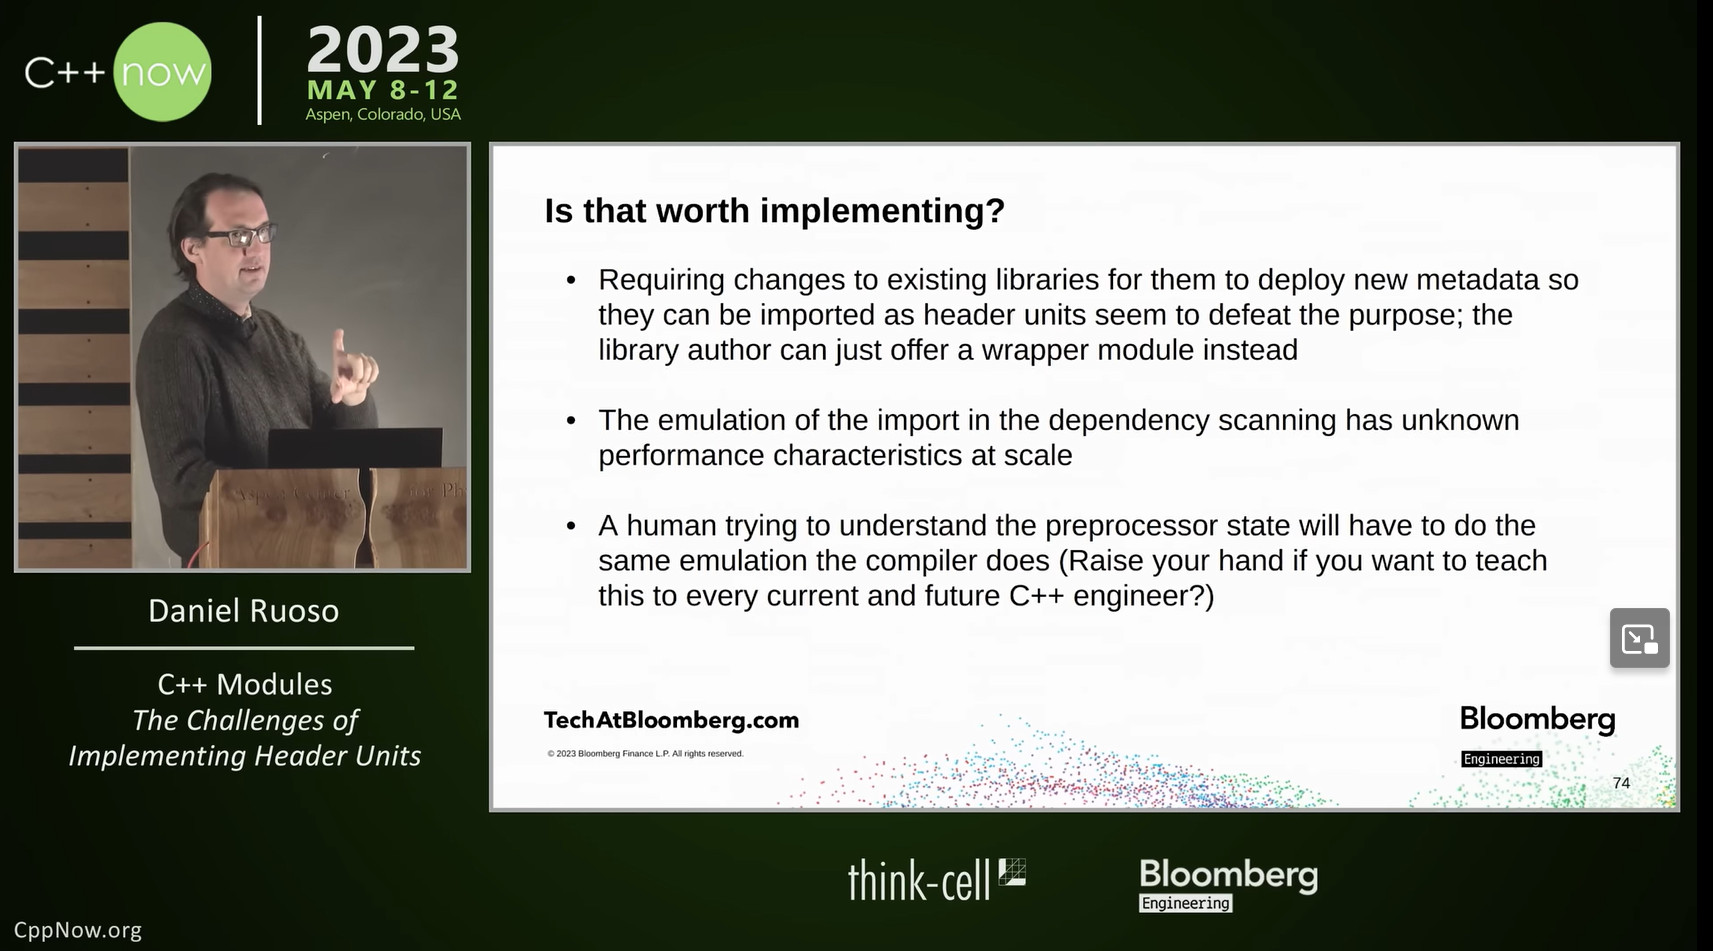
\includegraphics[height=.8\textheight]{modulesgfx/ruoso_header_units.jpg}}
  \end{center}
\end{frame}

\begin{frame}
  \frametitle{If you want to know more...}
  \begin{center}
    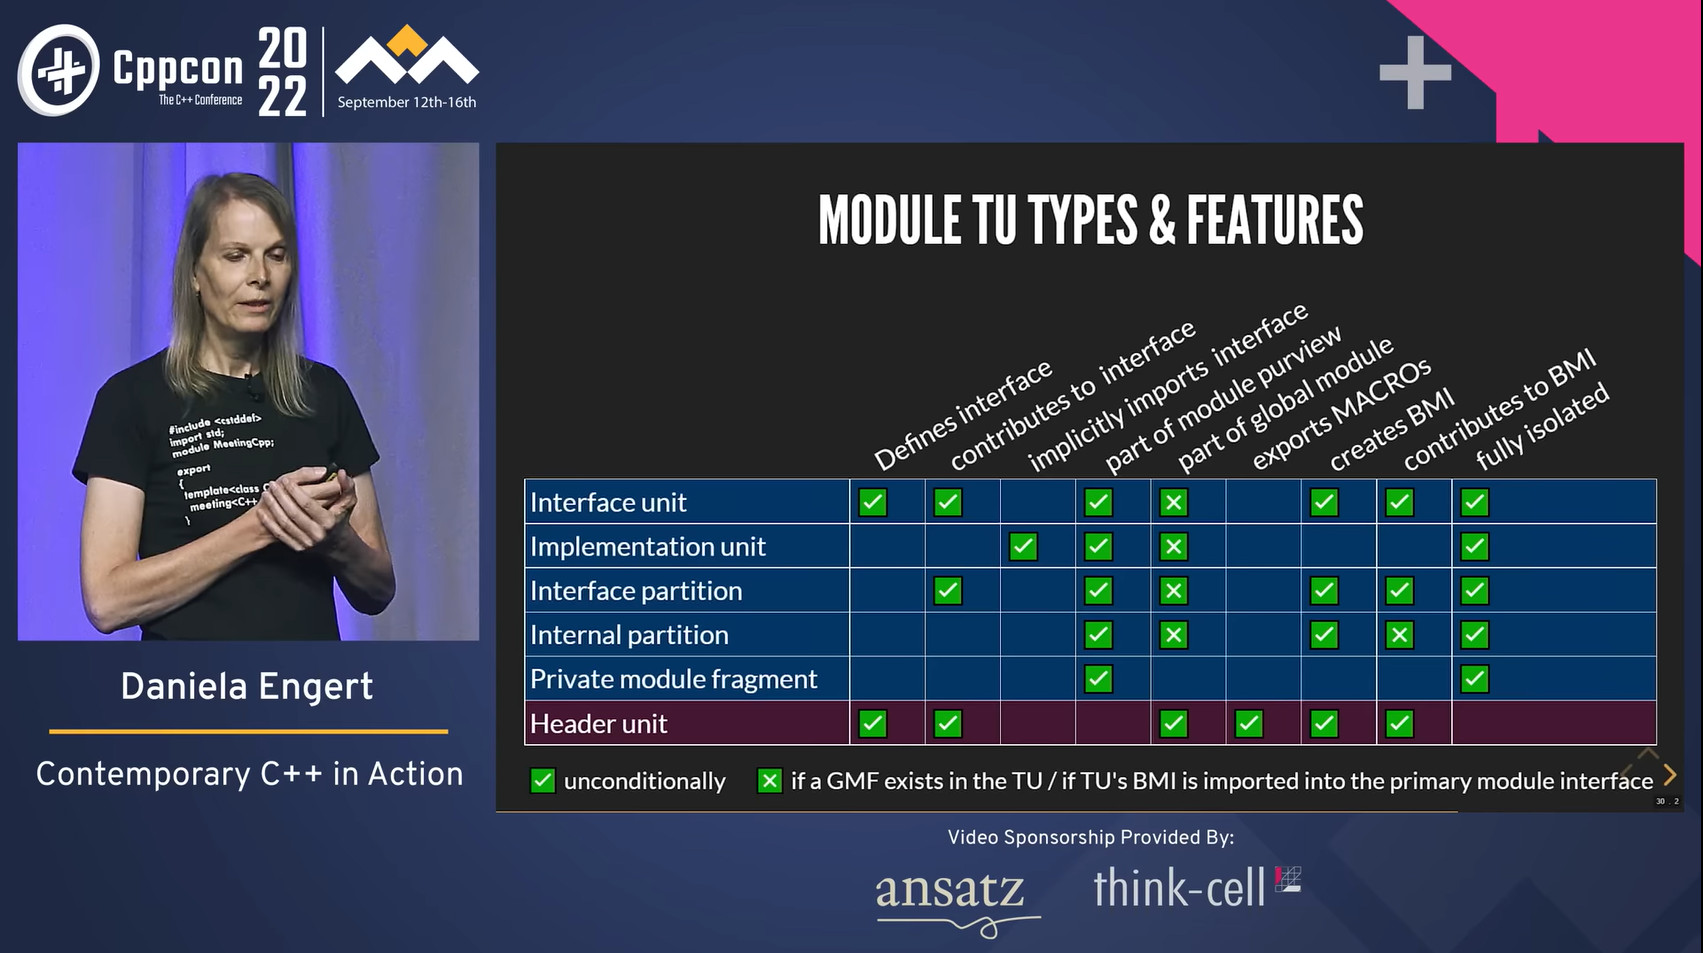
\includegraphics[height=.8\textheight]{modulesgfx/engert_table.jpg}
  \end{center}
\end{frame}


\begin{frame}[fragile]
  \frametitle{Building with CMake - Old School}

  \begin{lstlisting}[style=cmake]
cmake_minimum_required(VERSION 3.27)
project(my_project)

add_executable(my_executable)
target_sources(my_executable PUBLIC
  ${PROJECT_SOURCE_DIR}/my_src.cpp
  (*@\tmrk{a001}{}@*)${PROJECT_SOURCE_DIR}/inc/my_header1.hpp(*@\tmrk{b001}{}@*)
  (*@\tmrk{a002}{}@*)${PROJECT_SOURCE_DIR}/inc/my_header2.hpp(*@\tmrk{b002}{}@*)
)
target_include_directories(my_executable PUBLIC
  (*@\tmrk{a003}{}@*)${PROJECT_SOURCE_DIR}/inc(*@\tmrk{b003}{}@*))
  \end{lstlisting}

  \cuncover{2}{\tikz[overlay]\filldraw[blue, opacity=0.3] ([shift={(0,-0.5ex)}]a001) rectangle ([shift={(0,2ex)}]b001);}
  \cuncover{2}{\tikz[overlay]\filldraw[blue, opacity=0.3] ([shift={(0,-0.5ex)}]a002) rectangle ([shift={(0,2ex)}]b002);}
  \cuncover{3-}{\tikz[overlay]\filldraw[blue, opacity=0.3] ([shift={(0,-0.5ex)}]a003) rectangle ([shift={(0,2ex)}]b003);}
\end{frame}


\begin{frame}[fragile]
  \frametitle{Building with CMake - File Sets (since v3.23)}

  \begin{lstlisting}[style=cmake]
cmake_minimum_required(VERSION 3.27)
project(my_project)

add_executable(my_executable)
target_sources(my_executable PUBLIC
    ${PROJECT_SOURCE_DIR}/my_src.cpp
  PUBLIC
  (*@\tmrk{a010}{}@*)FILE_SET HEADERS(*@\tmrk{b010}{}@*)
  (*@\tmrk{a011}{}@*)BASE_DIRS(*@\tmrk{b011}{}@*) ${PROJECT_SOURCE_DIR}/inc
  (*@\tmrk{a012}{}@*)FILES(*@\tmrk{b012}{}@*)
    ${PROJECT_SOURCE_DIR}/inc/my_header1.hpp
    ${PROJECT_SOURCE_DIR}/inc/my_header2.hpp
)
  \end{lstlisting}
  
  \tikz[overlay]\filldraw[blue, opacity=0.3] ([shift={(0,-0.5ex)}]a010) rectangle ([shift={(0,2ex)}]b010);
  \tikz[overlay]\filldraw[blue, opacity=0.3] ([shift={(0,-0.5ex)}]a011) rectangle ([shift={(0,2ex)}]b011);
  \tikz[overlay]\filldraw[blue, opacity=0.3] ([shift={(0,-0.5ex)}]a012) rectangle ([shift={(0,2ex)}]b012);

\end{frame}

\begin{frame}[fragile]
  \frametitle{Building with CMake - Modules (experimental as of v3.37)}

  \begin{lstlisting}[style=cmake]
cmake_minimum_required(VERSION 3.27)
project(my_project)
set((*@\tmrk{a015}{}@*)CMAKE_CXX_STANDARD 20(*@\tmrk{b015}{}@*))

add_executable(my_executable)
target_sources(my_executable PUBLIC
    ${PROJECT_SOURCE_DIR}/my_src.cpp
  PUBLIC
  (*@\tmrk{a010}{}@*)FILE_SET MODULES(*@\tmrk{b010}{}@*)
  (*@\tmrk{a011}{}@*)BASE_DIRS(*@\tmrk{b011}{}@*) ${PROJECT_SOURCE_DIR}/mod
  (*@\tmrk{a012}{}@*)FILES(*@\tmrk{b012}{}@*)
    ${PROJECT_SOURCE_DIR}/mod/my_module.cpp
)
  \end{lstlisting}
  
  \tikz[overlay]\filldraw[blue, opacity=0.3] ([shift={(0,-0.5ex)}]a010) rectangle ([shift={(0,2ex)}]b010);
  %\tikz[overlay]\filldraw[blue, opacity=0.3] ([shift={(0,-0.5ex)}]a011) rectangle ([shift={(0,2ex)}]b011);
  %\tikz[overlay]\filldraw[blue, opacity=0.3] ([shift={(0,-0.5ex)}]a012) rectangle ([shift={(0,2ex)}]b012);
  \tikz[overlay]\filldraw[blue, opacity=0.3] ([shift={(0,-0.5ex)}]a015) rectangle ([shift={(0,2ex)}]b015);

\end{frame}

\begin{frame}[fragile]
  \frametitle{Some boilerplate required...}
  
  CMake Modules support is currently experimental. The details are boring and bound to change quickly.
  
  Refer to \underline{\href{https://stackoverflow.com/questions/57300495/how-to-use-c20-modules-with-cmake/61244367\#61244367}{https://t.ly/Dl8yE}} for the current state.
  
  For CMake 3.27 add:
  
  \begin{lstlisting}[style=cmake]
set(CMAKE_EXPERIMENTAL_CXX_MODULE_CMAKE_API
  aa1f7df0-828a-4fcd-9afc-2dc80491aca7)
  \end{lstlisting}
  For Clang you may also need to add:
  \begin{lstlisting}[style=cmake]
  set(CMAKE_CXX_EXTENSIONS OFF)
  \end{lstlisting}
\end{frame}

\begin{frame}
  \frametitle{Use the latest tools!}
  
  \begin{itemize}
  \item Absolute latest CMake (3.27)
  \item Latest Visual Studio 2022 (at least 19.34)
  \item Ninja 1.11
  \item Clang at least 16, prefer trunk
  \item gcc trunk, still without dependency scanning
  \end{itemize}
  
  Even with the latest tools there are still plenty of bugs and inconsistent behaviour between compilers!
\end{frame}


\begin{frame}[fragile]

  \frametitle{A few things to keep in mind}
  
  Module source file or regular source file?
  \begin{itemize}
  \item If it has an \texttt{export module} somewhere $\rightarrow$ Module
  \item If it is a module partition $\rightarrow$ Module
  \item Otherwise $\rightarrow$ Regular.
  \end{itemize}

  \cpause
  Which file extension?
  \begin{itemize}
  \item Many different extensions started appearing in the compilers: \texttt{.ixx}, \texttt{.cppm}, \texttt{.cxxm}, \texttt{.c++m}, \texttt{.ccm}.
  \item With CMake you don't need to use any of them!
  \item If you decide to use them, be sure to \textit{only} use them for module source files (as defined above)
  \end{itemize}
\end{frame}

\iffalse %!!!!!!!!!!!!!!!!!
\fi %!!!!!!!!!!!!!!!!!

\begin{frame}[fragile]
  \frametitle{What is a build system anyway?}

  \begin{lstlisting}
$ g++ -o my_src.o -I . -c my_src.cpp

$ g++ my_executable.o -o my_executable
  \end{lstlisting}
\end{frame}

\begin{frame}

  \frametitle{Tracking dependencies}

  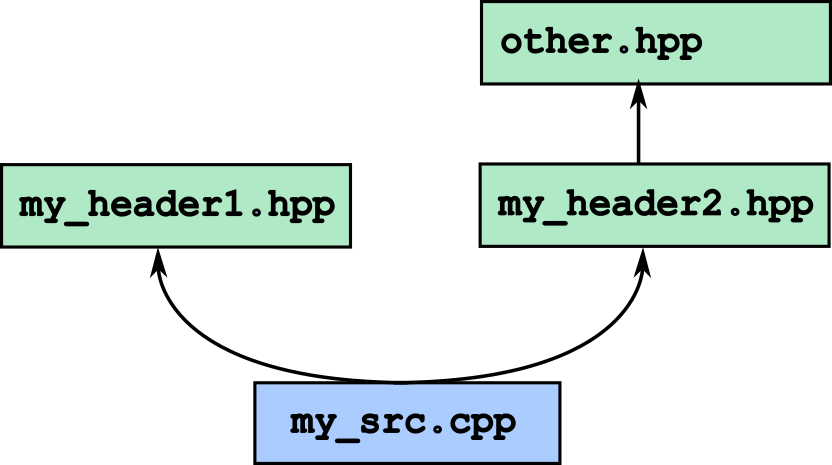
\includegraphics[height=.75\textheight]{modulesgfx/headers_dep_001.png}
\end{frame}

\begin{frame}[fragile]
  \begin{lstlisting}
$ g++ -o my_src.o.deps -I . -M -c my_src.cpp
  \end{lstlisting}
  
  \cpause
  
  --- \textit{File:} \texttt{my\_src.o.deps}
  \begin{lstlisting}
my_src.o: my_src.cpp \
  my_header1.hpp
  my_header2.hpp
  other.hpp
  \end{lstlisting}
\end{frame}


\begin{frame}
  \begin{center}
  \only<2>{\frametitle{What changes for the build system?}}
    \only<1>{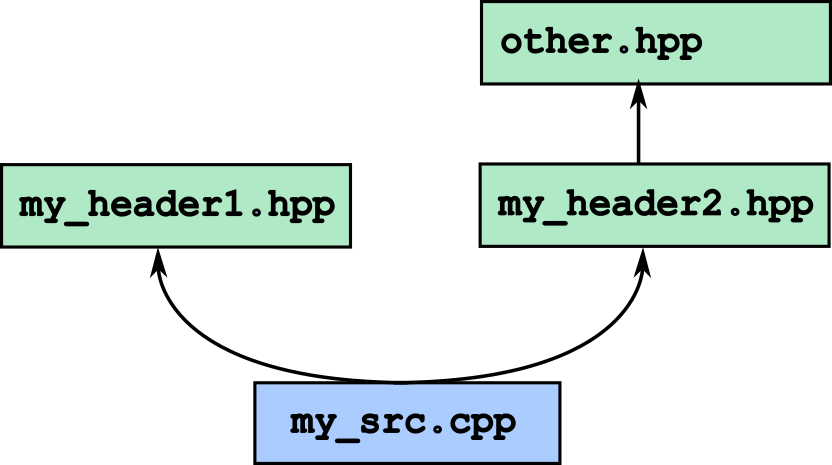
\includegraphics[height=.75\textheight]{modulesgfx/headers_dep_001.png}}
    \only<2>{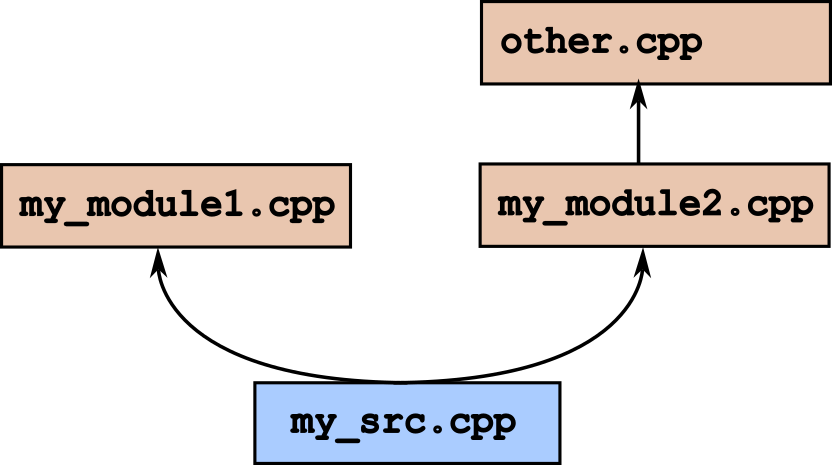
\includegraphics[height=.75\textheight]{modulesgfx/modules_dep_001.png}}
  \end{center}
\end{frame}

\begin{frame}[fragile]
  \frametitle{What changes for the build system?}
  
    \begin{lstlisting}[style=cmake]
add_executable(my_executable)
target_sources(my_executable PUBLIC
    ${PROJECT_SOURCE_DIR}/my_src.cpp
  PUBLIC
  FILE_SET MODULES
  BASE_DIRS ${PROJECT_SOURCE_DIR}
  FILES
    (*@\tmrk{a050}{}@*)${PROJECT_SOURCE_DIR}/my_module1.cpp (*@\tmrk{b050}{}@*)
    (*@\tmrk{a051}{}@*)${PROJECT_SOURCE_DIR}/my_module2.cpp (*@\tmrk{b051}{}@*)
    (*@\tmrk{a052}{}@*)${PROJECT_SOURCE_DIR}/other.cpp      (*@\tmrk{b052}{}@*)
)
  \end{lstlisting}
  
  \tikz[overlay]\filldraw[blue, opacity=0.3] ([shift={(0,-0.5ex)}]a050) rectangle ([shift={(0,2ex)}]b050);
  \tikz[overlay]\filldraw[blue, opacity=0.3] ([shift={(0,-0.5ex)}]a051) rectangle ([shift={(0,2ex)}]b051);
  \tikz[overlay]\filldraw[blue, opacity=0.3] ([shift={(0,-0.5ex)}]a052) rectangle ([shift={(0,2ex)}]b052);

  \note{
  \begin{itemize}
  \item Source Files are listed individually, instead of directory
  \item We don't want to model dependencies
  \end{itemize}
  }
\end{frame}

\begin{frame}
  \begin{center}
  \frametitle{What changes for the build system?}
    \only<1>{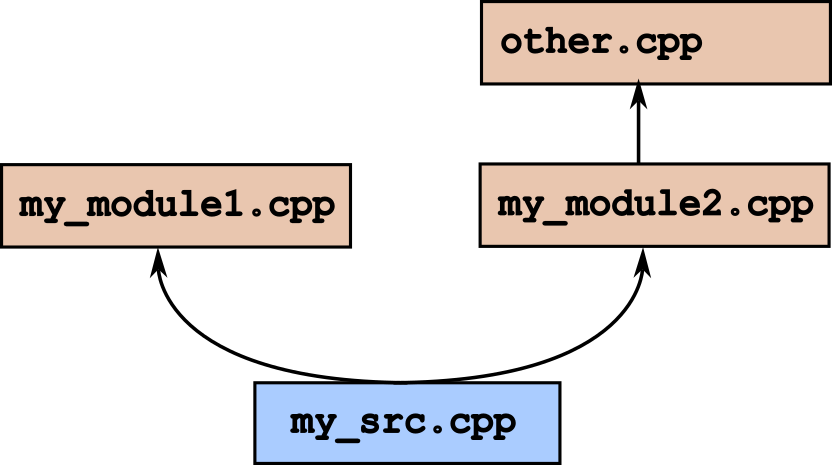
\includegraphics[height=.75\textheight]{modulesgfx/modules_dep_001.png}}
    \only<2>{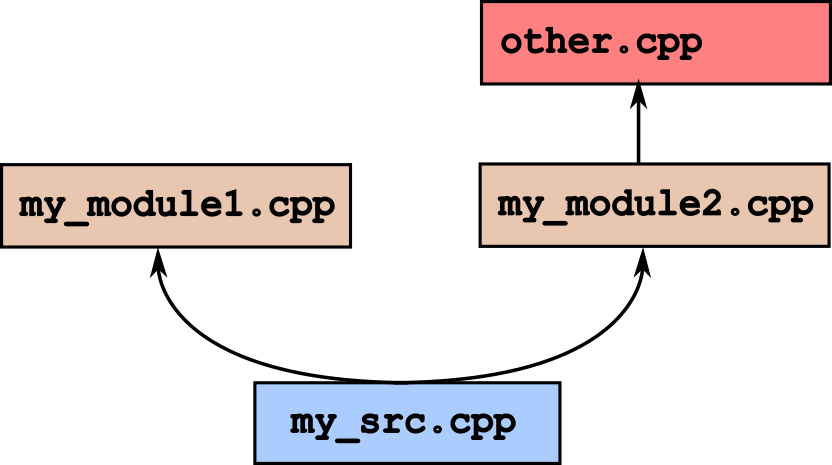
\includegraphics[height=.75\textheight]{modulesgfx/modules_dep_002.png}}
  \end{center}
\end{frame}


\begin{frame}[fragile]
  \frametitle{Interacting with headers - the global module fragment}
  
  \begin{onlyenv}<1-2>
  \begin{lstlisting}[style=cpp20]
export module A;

(*@\tmrk{a060}{}@*)import std;(*@\tmrk{b060}{}@*)

std::vector<int> getVector() {
  return std::vector<int>{ 1, 2, 3, 4 };
}
  \end{lstlisting}
  \end{onlyenv}
  
  \only<2>{
  \tikz[overlay]\filldraw[blue, opacity=0.3] ([shift={(0,-0.5ex)}]a060) rectangle ([shift={(0,2ex)}]b060);
  }
  
  \begin{onlyenv}<3-4>
  \begin{lstlisting}[style=cpp20]
(*@\tmrk{a061}{}@*)module;(*@\tmrk{b061}{}@*)

#include <vector>

(*@\tmrk{a062}{}@*)export module A;(*@\tmrk{b062}{}@*)

std::vector<int> getVector() {
  return std::vector<int>{ 1, 2, 3, 4 };
}
  \end{lstlisting}
  \end{onlyenv}
  \only<4>{
  \tikz[overlay]\filldraw[blue, opacity=0.3] ([shift={(0,-0.5ex)}]a061) rectangle ([shift={(0,2ex)}]b061);
  \tikz[overlay]\filldraw[blue, opacity=0.3] ([shift={(0,-0.5ex)}]a062) rectangle ([shift={(0,2ex)}]b062);
  }
\end{frame}

\begin{frame}[fragile]
  \frametitle{Beware of mixing headers and modules}
  --- \textit{File:} \texttt{my\_module.cpp}
  \begin{lstlisting}[style=cpp20]
export module m;

import std;

export std::string f() { return "!"; }
  \end{lstlisting}
  \cpause
  --- \textit{File:} \texttt{main.cpp}
  \begin{onlyenv}<1-2>
  \begin{lstlisting}[style=cpp20]
import m;


int main() {
  auto const s = f();
}
  \end{lstlisting}
  \end{onlyenv}
  \begin{onlyenv}<3>
  \begin{lstlisting}[style=cpp20]
import m;


int main() {
  std::string const s = f();
}
  \end{lstlisting}
  \end{onlyenv}
  \begin{onlyenv}<4>
  \begin{lstlisting}[style=cpp20]
import m;
#include <string>

int main() {
  std::string const s = f();
}
  \end{lstlisting}
  \end{onlyenv}
\end{frame}

\begin{frame}[fragile]
  \frametitle{Modularizing legacy libraries - Include standard library early}
  --- \textit{File:} \texttt{lib.hpp}
  \begin{lstlisting}[style=cpp20]
#include <string>
std::string f();
  \end{lstlisting}

  \begin{onlyenv}<1>
  --- \textit{File:} \texttt{libm.cpp}
  \begin{lstlisting}[style=cpp20]



export module lib;
export {
#include <lib.hpp>
}
  \end{lstlisting}
  \end{onlyenv}

  \begin{onlyenv}<2>
  --- \textit{File:} \texttt{libm.cpp}
  \begin{lstlisting}[style=cpp20]
module;
#include <string>

export module lib;
export {
#include <lib.hpp>
}
  \end{lstlisting}
  \end{onlyenv}
\end{frame}

\begin{frame}[fragile]
  \frametitle{Modularizing legacy libraries - Export names with \texttt{using}}

  --- \textit{File:} \texttt{lib.hpp}
  \begin{lstlisting}[style=cpp20]
class AwesomeType;
  \end{lstlisting}
  --- \textit{File:} \texttt{libm.cpp}
  \begin{lstlisting}[style=cpp20]
module;
#include <lib.hpp>
export module lib;
using ::AwesomeType;
  \end{lstlisting}
\end{frame}

\begin{frame}[fragile]
  \frametitle{Modularizing legacy libraries - Preprocessor macros}
  
  --- \textit{File:} \texttt{libm.cpp}
  \begin{lstlisting}[style=cpp20]
export module lib;
#define AWESOME_MACRO 42
  \end{lstlisting}
  
  --- \textit{File:} \texttt{main.cpp}
  \begin{lstlisting}[style=cpp20]
import lib;

int main() {
  return AWESOME_MACRO;  // error! macros cannot be exported
}
  \end{lstlisting}
\end{frame}

\begin{frame}[fragile]
  \frametitle{Modularizing legacy libraries - Preprocessor macros}
  
  --- \textit{File:} \texttt{libm.cpp}
  \begin{lstlisting}[style=cpp20]
export module lib;
// ...
  \end{lstlisting}
  
  --- \textit{File:} \texttt{libm.hpp}
    \begin{lstlisting}[style=cpp20]
#define AWESOME_MACRO 42
  \end{lstlisting}
  
  --- \textit{File:} \texttt{main.cpp}
  \begin{lstlisting}[style=cpp20]
import lib;
#include <libm.hpp>

int main() {
  return AWESOME_MACRO;
}
  \end{lstlisting}
\end{frame}


\begin{frame}[fragile]
  \frametitle{Modularizing legacy libraries - Preprocessor macros}
  
  --- \textit{File:} \texttt{libm.cpp}
  \begin{lstlisting}[style=cpp20]
export module lib;
#define AWESOME_MACRO 42
export constexpr int AwesomeConstant = AWESOME_MACRO;
  \end{lstlisting}
  
  --- \textit{File:} \texttt{main.cpp}
  \begin{lstlisting}[style=cpp20]
import lib;

int main() {
  return AwesomeConstant;
}
  \end{lstlisting}
\end{frame}

\begin{frame}
  \frametitle{Daniela Engert - Contemporary C++ in Action}
  \begin{center}
    \href{https://www.youtube.com/watch?v=yUIFdL3D0Vk}
    {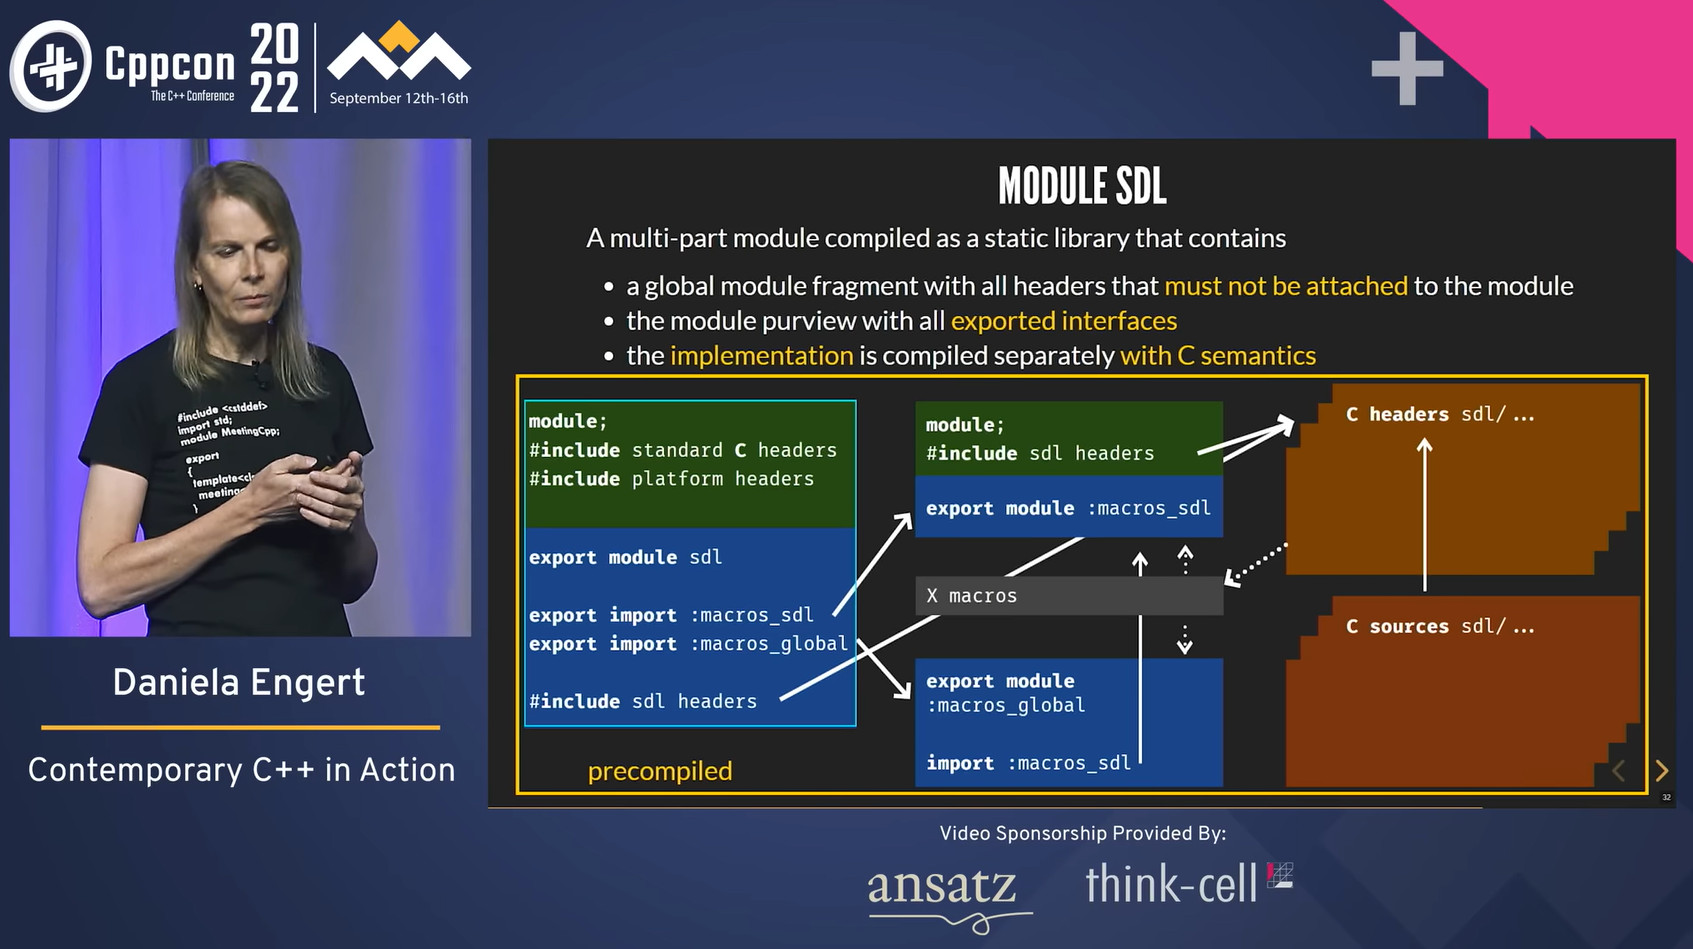
\includegraphics[height=.8\textheight]{modulesgfx/engert_contemporary.jpg}}
  \end{center}
\end{frame}


\begin{frame}
  \frametitle{Conclusion}
  
  \begin{itemize}
  \item Modules are slowly maturing. Try them out today!
  \item There is still a lot of dark corners in the implementations, but the more people use them, the quicker those get fixed.
  \item Integrating header-based legacy code is challenging and requires some practice.
  \end{itemize}
  
  \note{
  \textbf{TIMECHECK}: 0:55
  }
\end{frame}

\begin{frame}
  \frametitle{Thanks for your attention.}

  \href{https://stackoverflow.com/users/577603/comicsansms}{
\includegraphics[height=.05\textheight]{resources/so-icon.png}}
  \href{https://github.com/ComicSansMS}{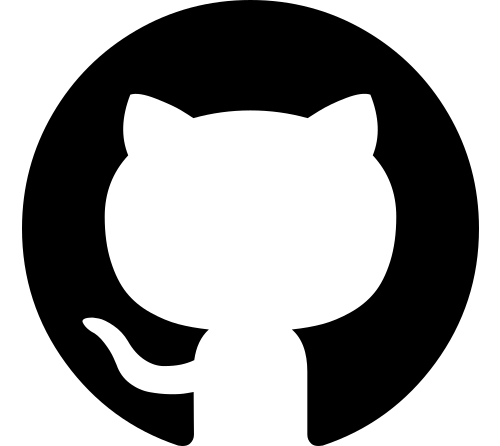
\includegraphics[height=.05\textheight]{resources/github-icon.png}}
  \includegraphics[height=.05\textheight]{resources/discord-icon.png} Andreas Weis
\end{frame}


\end{document}
